\section{Method}

This section details the feature extraction process, model architectures, and training procedures used for respiratory phase classification. The overall feature extraction pipeline is illustrated in Fig.~\ref{fig:feat_ext_diagram}.


\begin{figure}[h!]
\centering
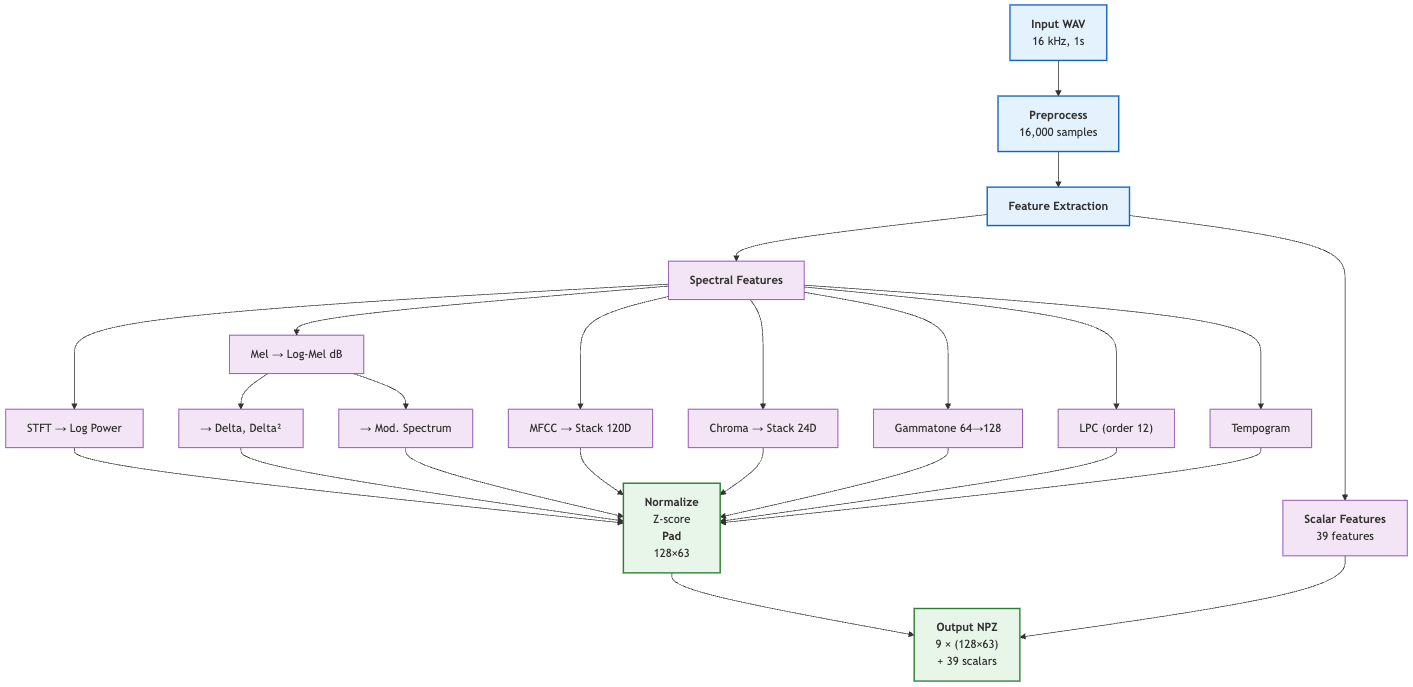
\includegraphics[width=\columnwidth]{figures/feature_extraction}	
\caption{Feature extraction pipeline diagram}
\label{fig:feat_ext_diagram}
\end{figure}

\subsection{Feature Extraction}

The input to our system is a one-second audio clip sampled at 16 kHz. From each clip, we extracted two categories of features: spectral representations and scalar values. All features were pre-computed and stored as NumPy archives to accelerate the training pipeline.

\subsubsection{Spectral Representations}

We computed nine distinct time-frequency representations: STFT, Mel-spectrogram with its first (delta) and second (delta-delta) derivatives, Mel-Frequency Cepstral Coefficients (MFCC), chroma, gammatone, modulation spectrum, and tempogram. Visual comparisons for these features are provided in Figs.~\ref{fig:stft}-\ref{fig:tempogram}. All spectral features were reshaped or padded to a uniform dimension of 128 frequency bins by 63 time steps and were normalized using z-scoring.

\begin{figure}[h!]
\centering
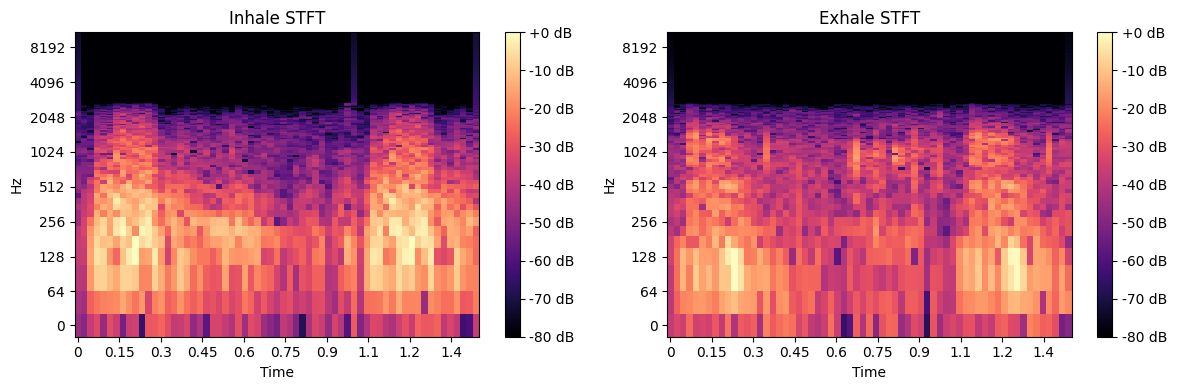
\includegraphics[width=\columnwidth]{figures/stft}	
\caption{STFT spectrograms for inhale/exhale}
\label{fig:stft}
\end{figure}

\begin{figure}[h!]
\centering
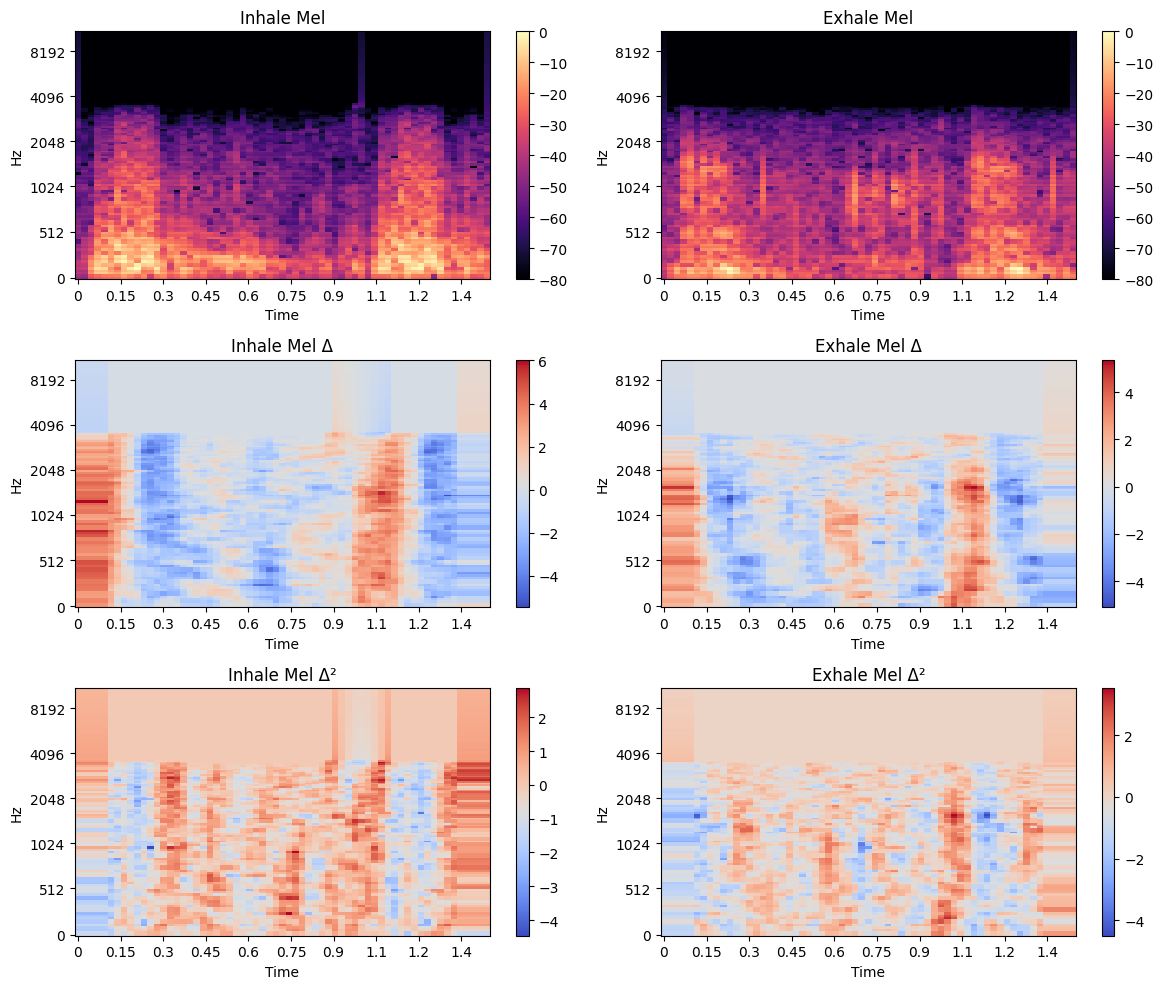
\includegraphics[width=\columnwidth]{figures/mel}	
\caption{Mel spectrograms with delta coefficients}
\label{fig:mel}
\end{figure}

\begin{figure}[h!]
\centering
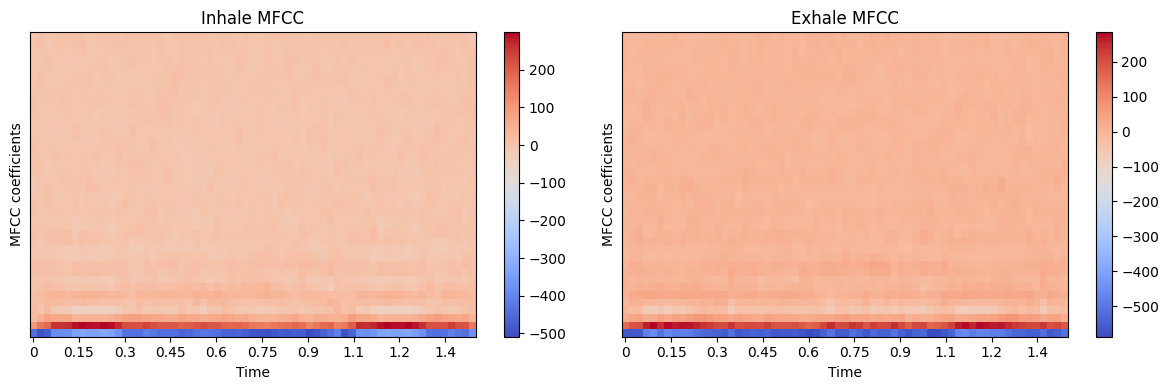
\includegraphics[width=\columnwidth]{figures/mfcc}	
\caption{MFCC comparison}
\label{fig:mfcc}
\end{figure}

\begin{figure}[ht!]
\centering
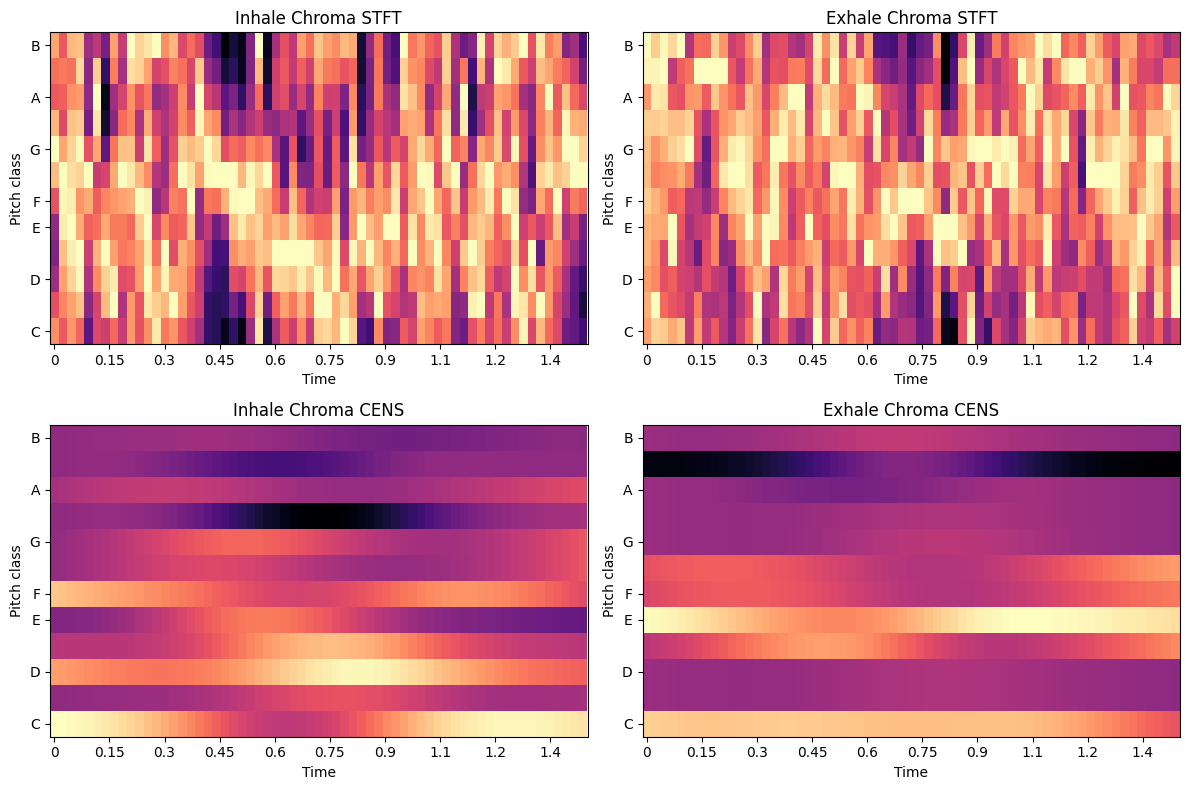
\includegraphics[width=\columnwidth]{figures/chroma}	
\caption{Chroma STFT and CENS features}
\label{fig:chroma}
\end{figure}

\begin{figure}[h!]
\centering
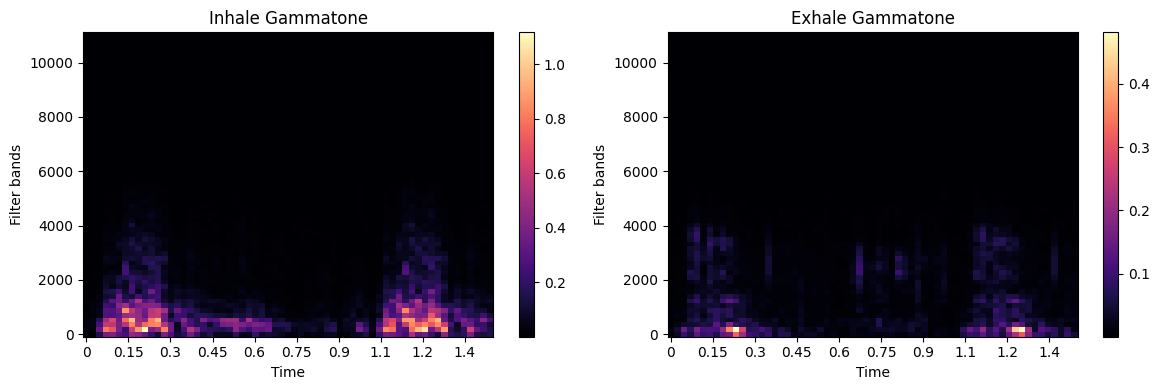
\includegraphics[width=\columnwidth]{figures/gammatone}	
\caption{Gammatone filterbank features}
\label{fig:gammatone}
\end{figure}

\begin{figure}[h!]
\centering
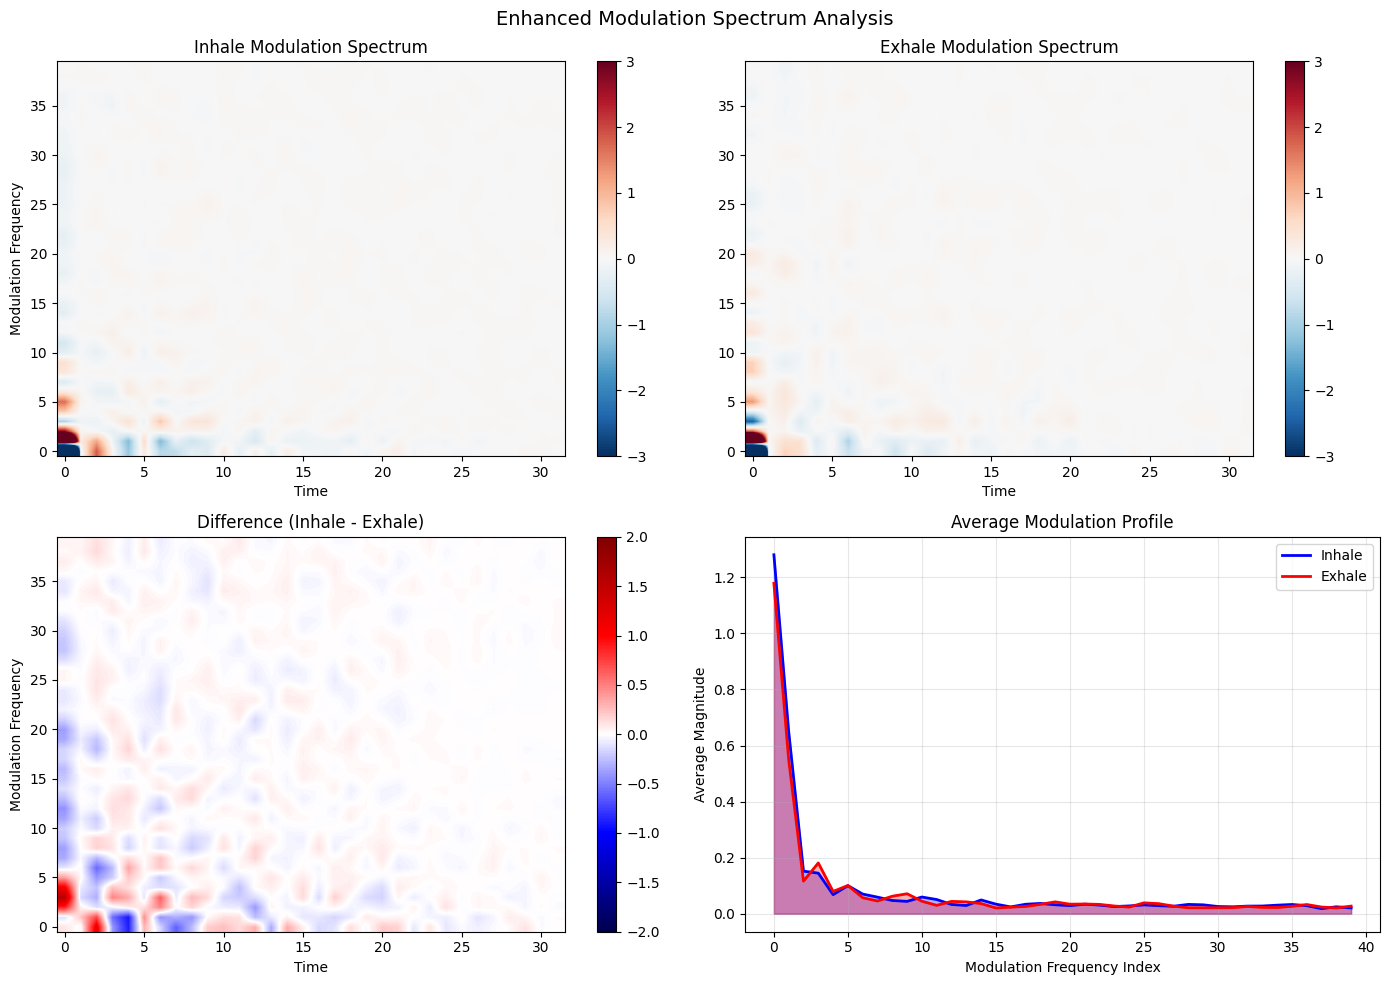
\includegraphics[width=\columnwidth]{figures/modulation}	
\caption{Modulation spectrum analysis}
\label{fig:modulation}
\end{figure}

\begin{figure}[h!]
\centering
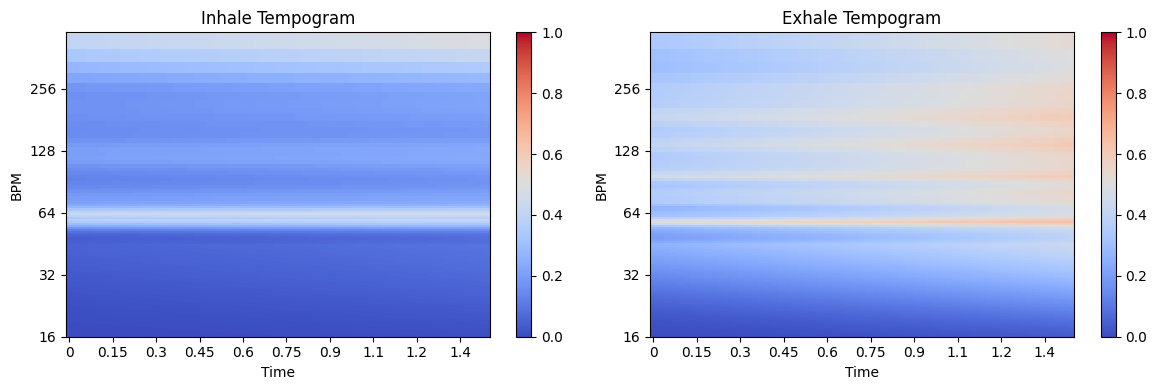
\includegraphics[width=\columnwidth]{figures/tempogram}	
\caption{Tempogram comparison}
\label{fig:tempogram}
\end{figure}

\subsubsection{Scalar Features}

We extracted 39 scalar features---spanning temporal metrics (e.g., RMS energy, ZCR) and spectral statistics (e.g., centroid, bandwidth)---to characterize the signal. Key feature comparisons between respiratory phases are plotted in Fig.~\ref{fig:scalars}.

\begin{figure}[h!]
\centering
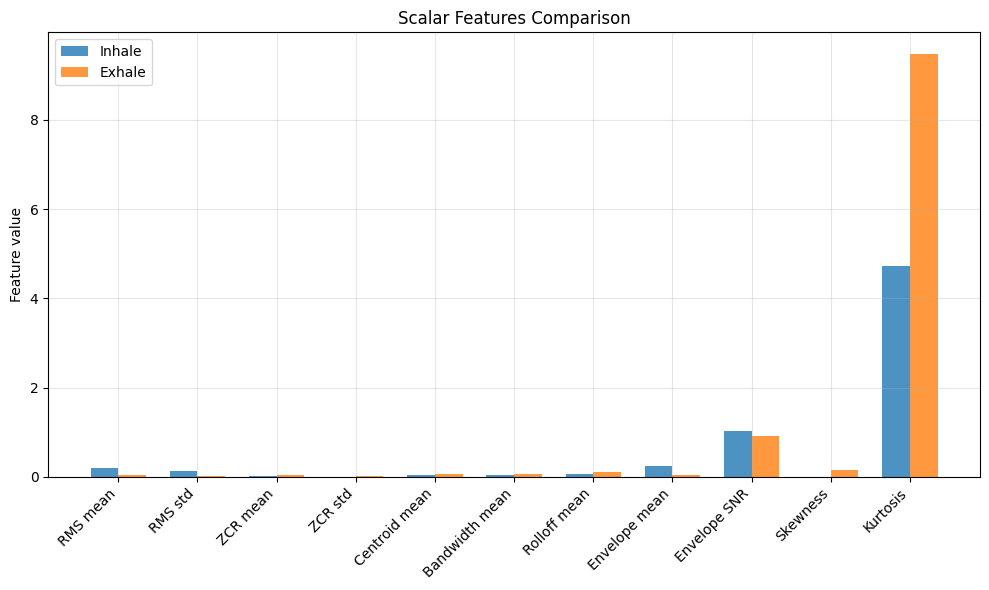
\includegraphics[width=0.9\columnwidth]{figures/scalars}	
\caption{Scalar features comparison}
\label{fig:scalars}
\end{figure}

\subsection{Model Architectures}

We designed two Convolutional Neural Network (CNN) architectures to process the combined feature sets. Each model contains a convolutional pathway for spectral features and a Multi-Layer Perceptron (MLP) pathway for scalar features.

\subsubsection{CNN8}

This is a lightweight model with eight convolutional layers organized in four blocks ($32\rightarrow64\rightarrow128\rightarrow256$ channels). It uses ReLU activations, Batch Normalization, and max pooling. The scalar pathway is a two-layer MLP.

\subsubsection{VGG-Inspired Model}

This higher-capacity model contains 12 convolutional layers in four blocks ($64\rightarrow128\rightarrow256\rightarrow512$ channels) with GELU activations. A residual connection is included in the final block. The model contains 8.15M trainable parameters.

\subsection{Training and Optimization}

\subsubsection{Optimizer}

Models were trained with the \textit{AdamW} optimizer using a weight decay, $\lambda$ of $10^{-4}$ . The learning rate followed a cosine annealing schedule with a linear warmup. Initial learning rates were set to $4\times10^{-4}$ for CNN8 and $1\times10^{-3}$ for the VGG-inspired model. Gradient norms were clipped at a maximum value of $1.0$.

\subsubsection{Data Augmentation}

After a four-epoch warmup, we applied stochastic data augmentation. The methods used were \textit{CutMix}, with a probability of 0.6, and \textit{MixUp}, with a probability of 0.4.

\subsubsection{Training Configuration}

We used a binary cross-entropy with logits loss function. The data was split into training (80\%) and validation (20\%) sets using a stratified method. Training ran for a maximum of 140 epochs with early stopping based on validation accuracy. Mixed-precision training was used to reduce computation time.

\subsection{Ensemble Method}

Final predictions for the test set were generated by an ensemble of the trained models. The sigmoid outputs of the models were combined using a weighted average, as shown in (1).

$$P_{\text{final}} = \sum_{i=1}^{N} \alpha_i \cdot \sigma(\text{logits}_i) \eqno{(1)}$$

The weights, $\alpha_i$ , were derived from the softmax-normalized validation accuracy of each contributing model, giving greater influence to better-performing models.
